%&platex --translate-file=cp1250pl
\documentclass[times]{jtitauth}

\begin{document}

\title{Control of the effects of crystal\\
dispersion at different orders in the mixing\\
of three phase-matched waves\\
on a 5- to 100-fs time scale}

\author{Alessandra Andreoni,  Maria Bondani, and Marco A.C. Potenza}

\markboth{Alessandra Andreoni,  Maria Bondani, and Marco A.C. Potenza}
{Control of the effects of crystal
dispersion at different orders in the mixing
of three phase-matched waves
on a 5- to 100-fs time scale}

\maketitle

\begin{abstract}
A number of manners to obtain first-order achromatic phase
mat\-ching  of both type I and type II are presented and the most
advantageous ones are identified to generate high-spectral quality
100-fs pulses by either parametric generation or frequency
up-conversion. In the case of frequency-doubling high-energy 5-fs
Ti:sapphire pulses, a non-collinear phase-matching I geometry in a
$\beta$-barium borate crystal cut at 44 deg is devised that should
allow high conversion efficiency, virtually without pulse
lengthening and intra-pulse frequency chirp due to group-velocity
dispersion.
\end {abstract}

\begin{keywords}
three-wave mixing, ultra-broadband phase-matching,
$\beta$-ba-rium borate, group-velocity matching, group-velocity
dispersion\
\end{keywords}

\section{First level section}

\subsection{Second level section}

To investigate optical nonlinearities of materials and structures
for ultra\-fast opto-optical and opto-electronic devices, it is
becoming more and more necessary to develop table-top solid-state
sources of high-power ultrashort pulses, broadly tunable in the
near-UV/visible range. Particularly, after refinements of the
chirped-pulse amplification (CPA) techniques led to
ultra-broadband amplifiers giving multiterawatt pulses, sources
based on optical parametric conversion/amplification, capable of
sustaining consistently broad bandwidths, received great
attention. Nowadays, harmonics of pulses with duration of the
order of 100~fs are thus rather extensively used, either as pump
pulses for parametric converters/amplifiers or in frequency-mixing
schemes. They are typically mixed with the IR-tunable output of
parametric generators pumped by the fundamental output of CPA
sources such as Ti:sapphire and Nd:glass lasers.

The large chromatic dispersion of all nonlinear crystals available
for these parametric interactions, however, makes generation of
blue and near-UV wavelengths very critical when the pulse duration
is 100~fs or less, in that also the minimal requirement in the
frequency domain (first-order achromatic phase matching) becomes
difficult to be fulfilled. In fact, only accidentally, the pump
wavelengths available from Ti:sapphire and Nd:glass lasers, or
from their harmonics, allow phase-matching (PM) with pulses at the
wavelengths of interest, collinearly propagating with group
velocities (GV's) sui\-tably matched for efficient energy
exchange. For type I phase-matching in $\beta-\textrm{BaBO}_4$
(BBO I), this occurs in spectral regions of the signal wave too
narrow to be useful when the pump is at short wavelengths. Broad
regions in which the GV's are mismatched by less than 100~fs/mm
exist for BBO II collinearly pumped at wavelengths between Nd
fundamental and its second harmonic (SH). The case of pump at the
Ti:sapphire fundamental represents a particularly fortunate
circumstance, in which signal and idler have opposite GV mismatch
(GVM) values with respect to the pump, of about 50~fs/mm in
magnitude, over a reasonably broad spectral region. Wilson and
Yakovlev [1] exploited it with success to amplify a fs near-IR
continuum with up to 45\% efficiency in 3- and 5-mm long BBO II
crystals and obtained broadly tunable high-energy pulses of
30-50~fs duration with frequency-conversion techniques in thin
crystals.

The problem of GVM is obviously also relevant to SH generation
itself on the 100-fs time scale [2-5]: for instance, when
Ti:sapphire high-energy pulses are frequency-doubled to pump
parametric converters/amplifiers, there is a~trend to circumvent
such problem by using thin crystals and high intensities of the
fundamental pulses. This attitude should be revised, according to
a recent and extended study of the various effects, which affect
the SH conversion efficiency in collinear PM I, pulse width and
intra-pulse spectral distribution~[5]. In fact, the interplay of
dispersion and nonlinear interactions leads to crystal lengths and
fundamental-pulse intensity values that are optimal for frequency
doubling Ti:sapphire pulses of 150~fs. More specifically, the
ana\-lysis carried out in  [5], which includes both
second-order-dispersion effects and third-order nonlinearities,
shows that, as soon as the crystal depth goes beyond the length of
the pathway over which fundamental and SH pulses keep superimposed
while travelling, the use of high intensities may turn out to be
disadvantageous. All experimental and theoretical results reported
in  [5] lead to the conclusion that the most critical effect in
both BBO and LBO (${\rm LiB_3O}_5$) is that related to first-order
dispersion.

A number of groups proposed a more fundamental approach to the
problem of GVM and developed interaction schemes that allow GVM
compensation [6$\div$12]. These schemes are obviously specific for
each nonlinear material and type of PM: while those developed for
high-quality SH generation must only couple the GV's of
fundamental and SH pulses [3$\div$7, 13], those for optimizing the
parametric interactions of pulses at three different wavelengths
can ensure the fulfillment of various GV matching conditions that
are all of interest. As to sum-frequency generation, schemes
linking the GV's of the pulses at $\omega_1$ and $\omega_2$ either
to each other or to ${\rm GV}_{\omega_1 + \omega_2}$ were
considered [8]. As to parametric generation/amplification, we
demonstrated both theoretically [14] and in a number of
experiments [9, 11, 12] that, in noncollinear PM geometries, the
excess in the signal and idler GV's with respect to the pump GV
can be cancelled, at each wavelength in the tuning range of the
crystal adopted, by a proper choice of the pump angles, {\it i.e.}
the angles of pump {\bf k}-vector, ${\rm{\bf k}}_p$, to crystal
axis. By using such a GVM-compensated travelling-wave BBO
generator to seed a collinear amplifier pumped by 120~$\mu$J
pulses at 0.4~$\mu$m, we demonstrated a 17\% conversion efficiency
into nearly transform-limited sub-100~fs pulses [15]. Since a
specific noncollinear configuration of the seeder works properly
in a tuning range that covers at most 100~nm, this approach,
though of rather general applicability [14], is not ideal for
obtaining a broadly tunable parametric source, but could be useful
for SH generation ({\it vide infra}). For parametric sources, it
is more interesting the collinear PM I configuration described in
[16]: here, GV compensation is achieved over the entire tuning
range of BBO by suitably tilting the pulse front of the
Ti:sapphire SH pulse used as the extra-ordinary pump. In fact, a
pump pulse, whose front is tilted by an angle $\gamma$ on the same
side of the walk-off angle $\rho$, exhibits a GV in the direction
of ${\rm \bf k}_p$ that is greater than that of an untilted pulse
by the amount $\Delta{\rm GV = GV} \tan \rho \tan \gamma$. We used
this effect to match the GV-component parallel to ${\rm \bf k}_p$
of the tilted pump pulse with the mean value of the GV's of the
signal and idler pulses, this condition granting that they can be
amplified while staying locked to the pump pulse, without
broadening or gain saturation [17, 18]. By using 100-fs SH
Ti:sapphire pump pulses, we thus obtained collinearly generated
superfluorescence pulses tu\-nable to wavelengths as short as
456~nm~[16]. Recently, we showed that these pulses could be
efficiently amplified, in the same BBO I crystal in which they are
generated with tilted pulse fronts, by using pump pulses with the
fronts tilted by the same $\gamma$ angle as before. The tilt of
the amplified signal pulses could be fully compensated. By
characterizing the output of the system as to pulse spectrum and
time profile, we found va\-lues of the time-bandwidth product
close to the Fourier limit for signal-pulse energies of up to
1.5~$\mu$J~[19].

A general conclusion concerning three-wave interactions in
crystals such as BBO, LiIO$_3$ and KH$_2$PO$_4$ (KDP) [14] as well
as LBO [5] can be drawn: pulses of duration of the order of 100~fs
and at almost any wavelengths in the tuning ranges of the crystals
can strongly interact because geometries can be generally devised
simultaneously producing phase-matching and GV-matching conditions
that ensure suitably broadband interaction. Furthermore, making
the pathway over which the three travelling pulses are
superimposed greater than the crystal length renders the
three-wave inter\-action unexpectedly insensitive to the effects
of dispersion at orders above the first one. All experiments
reported in the literature ({\it e.g.} [5, 9, 11, 12, 15, 16,
19]), in which the interaction is made to occur in such a
situation, show that transform-limited output pulses are observed
whenever the intense incident pulse is transform-limited.

In this paper, we report on what we consider a noticeable
application of an accurate cancellation of first-order dispersion
effects in BBO I and give useful criteria to  identify the best
operating conditions, as to first- and second-order dispersion
effects, for frequency-doubling Ti:sapphire laser pulses, as short
as those recently obtained [20, 21]. We find that the GVM arising
from first-order dispersion of BBO can be cancelled over such an
extended frequency range that efficient conversion to SH, without
noticeable pulse lengthening, can be obtained by using relatively
long crystals and hence fundamental pulses at non-extreme
intensities. This is so true that it becomes worthwhile to control
the frequency chirp due to GV dispersion (GVD), which is a second
order effect usually overcome by the chirp due to self-phase
modulation in travelling-wave up-conversion schemes.

In a noncollinear PM I geometry of SH generation, in which we call
$\theta$ the {\bf k}$_F$-to-{\bf k}$_{SH}$ angle inside BBO, the
value that ensures
\begin{equation}
{\rm GVM}_{F,SH} = \left({\rm GV}_F \cos \theta \right )^{-1} -
\left ({\rm GV}_{SH}\right)^{-1} = 0
\end{equation}
at $\lambda_ F$ = 0.79~$\mu$m is $\theta = 10.25$~deg and the PM
angle is $\alpha = 42$~deg (for calculations, see [14]). We first
observe that, if the crystal is cut at an angle equal to $\alpha$,
the two fundamental pulses entering the crystal at incidence
angles $\theta_{{\rm ext}} = \pm 17.1$~deg, which corresponds to
the desired value for the internal angle, $\theta$, undergo
pulse-front tilting by angles smaller than tenths of degree over a
spectral range as broad as that of a transform-limited 5-fs pulse.
Furthermore, due to the symmetric incidence of the two fundamental
beams, the SH pulse is generated untilted. It is worth noting that
the lateral spectral components of the Ti:sapphire pulse [20],
that we keep undispersed when entering the crystal, by travelling
at angles $\theta \neq 10.25$~deg, are likely to form distinct
wavepackets, no more exactly GV-matched with their
frequency-doubled counterparts. If we call $\lambda_{F}^*$ the
wavelength corresponding to the pulse central frequency, $\Omega$,
and $\alpha^* = \alpha \left(\lambda_{F}^*\right)$ and $\theta^* =
\theta \left(\lambda_{F}^* \right)$ the angles that verify Eq.~(1)
at $\lambda_{F}^*$, the internal angles at which the different
components travel are given by:
\begin{equation}
\begin{array}{rcl}
\displaystyle{\theta_{\rm int} \left(\lambda_F\right)} & = &
\displaystyle{\arcsin \left[ n_F
\left(\lambda_{F}^* \right) \sin \theta^* / n_F \left(\lambda_F
\right)\right]}\\
& = & \displaystyle{\arcsin \big [\sin \theta_{\rm ext} / n_F
(\lambda_F)\big]~.}
\end{array}
\end{equation}

This produces a fundamental-to-SH time-drift per millimeter, given
by
\begin{equation}
\begin{array}{rcl}
\displaystyle{d\big(\lambda_F\big)} & = & \displaystyle{\big[{\rm GV}_F (\lambda_F) \cos
\theta_{\rm int} (\lambda_F)\big]^{-1} +} \\
& & \displaystyle{- [{\rm GV}_{SH} (\alpha^*
\, , \lambda_F /2)]^{-1}~.}
\end{array}
\end{equation}

Since the dispersion of BBO is such that this effect is more
pronounced  at short than at long $\lambda_F$ values, to make the
effect minimal across the whole spectrum of a 5-fs fundamental
pulse, say between 0.7 and 0.85~$\mu$m~[20], it is convenient to
adopt a geometry optimised, for instance, at $\lambda_F^* =
0.76~\mu$m, instead of $0.79~\mu$m, which would correspond to
$\Omega$. According to our calculations, this amounts to taking
$\alpha^* = 44~{\rm deg}~(= \theta_{\rm cut})$ and $\theta^* =
10.72~{\rm deg}~(\theta_{\rm ext} = 18.0~{\rm deg})$.

\begin{figure}[!hbp]
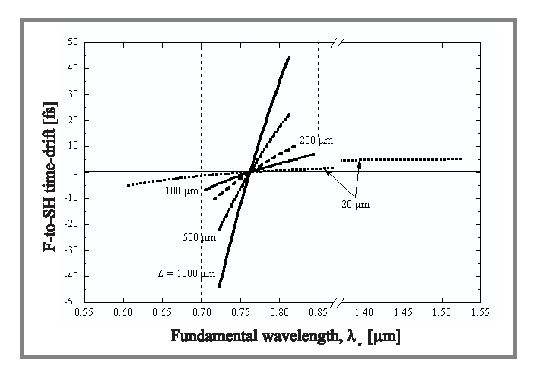
\includegraphics{fig}
\caption{Fundamental-to-SH time-drift in BBO I, at different
crystal depths, {\it L}, as a function of $\lambda_F$ in the
spectral range of Ti:sapphire, when SH generation occurs in
conditions of ideal GV-matching at $\lambda_F^* = 0.76~\mu{\rm m}$
%PB\\ The curves are plotted in the regions where the time-drift due
\hfill\break The curves are plotted in the regions where the time-drift due
to GVM is below the  time broadening due to GVD. The two vertical
dashed lines mark the positions of the lateral peaks in the
spectrum of the 5 fs pulse of Ref.~[20]}
\end{figure}
The fundamental-to-SH time-drift accumulated across different
BBO depths, {\it L}, are plotted in Fig.~1 as a function of
$\lambda_F$, in the range of Ti:sapphire: the drift is obviously
zero at 0.76~$\mu$m and increases, in magnitude, on going towards
the edges of the spectral range. In our opinion, it is reasonable
to accept time-drifts smaller than the duration with which an
incident pulse of full-width at half-maximum (FWHM) duration
$\tau_0 = 5$~fs would leave a BBO crystal of depth {\it L}, being
affected by pure GVD effects. We thus calculated such duration
values, $\tau (L)$, according to [22]:
\begin{equation}
\tau (L) = \tau_0 \sqrt{1 + \left( \left|\frac{\partial^2
k}{\partial\omega^2} \right|_\Omega 4\ln 2 \frac
{L}{\tau_0^2}\right)^2}
\end{equation}
\noindent in which
\begin{equation}
\left(\frac{\partial^2 k}{\partial \omega^2}\right)_\Omega = {\rm
GVD}_\Omega = - \frac 1 {\rm GV^2}\left(\frac{\partial {\rm
GV}}{\partial\omega} \right)_\Omega
\end{equation}
with GVD$_{\Omega (0.79 \mu{\rm m)}} \cong 76~{\rm fs}^2/{\rm mm}$
[23] and truncated the time-drift plots in Fig.~1 at $\pm\tau(L)$.
We observe that these plots extend over spectral regions that
broaden on decreasing {\it L}. This originates from the fact that,
on decreasing {\it L}, the time spread due to GVD, {\it i.e.}
$\tau(L) - \tau_0$, decreases less than linearly with {\it L},
whereas the fundamental-to-SH time-drift is proportional to {\it
L}. As a~result, a spectrum as broad as that comprised between 0.7
and 0.85~$\mu$m [20] becomes achieveable to SH generation with a
BBO I crystal of depth between 100 and 200~$\mu$m. Note that such
depth values, which allow keeping under control both first- and
second-order dispersion effects, are greater by one order of
magnitude than the distance over which first-order dispersion
effects are negligible in collinear SH generation [5]. Finally,
the fact that, in our noncollinear geometry, the fundamental- and
SH- pulses are perfectly GV-matched in the direction of {\bf
k}$_{SH}$ around their central frequencies, ensures that the
strongest field-components experience the strongest coupling and
hence produces a sort of locking of the interacting pulses [8, 9,
12, 24]. We are also confident that the concomitant absence of
pulse-front tilt and negligibility of higher-order nonlinear phase
shifts in BBO up to intensities well above 100 GW/cm$^2$ [5]
should limit the effects of first- and second-order dispersion
below those shown in Fig.~1 for the SH intrapulse-frequency chirp.


\section*{Acknowledgements}

The authors are deeply indebted to all co-authors of the papers
quoted, which testify many fruitful long-lasting cooperations.
This work was supported by the Italian National Research Council
(C.N.R.) through grants 96.00264.CT02~and~97.00070.CT02.~M. A. C.
Potenza acknowledges E.N.E.A. (Ente per le Nuove Tecnologie,
l'Energia e l'Ambiente) for his PhD studentship.

\begin{thebibliography}{99}
\bibitem{1}K. R. Wilson and V. V. Yakovlev, ,,Ultrafast rainbow: tunable ultrashort
 pulses from a solid-state kilohertz system'', {\it J. Opt. Soc. Am. B}, vol. 14, pp. 444--448, 1997.
\bibitem{2}J. Comly and E. Garmire, ,,Second harmonic generation from short
pulses'', {\it Appl. Phys. Lett.}, vol. 12, no. 7-9, 1968.
\bibitem{3}O. E. Martinez, ,,Achromatic phase matching for second harmonic ge\-neration
of femtosecond pulses'', {\it IEEE J. Quant. Electron.}, vol.
QE-25, pp. 2464--2468, 1989.
\bibitem{4}G. Szabo and Z. Bor, ,,Broadband frequency doubler for
femtosecond pulses'', {\it Appl. Phys. B}, vol. 50, pp. 51--54,
1990.
\bibitem{5}J.-Y. Zhang, J. Y. Huang, H. Wang, K. S. Wong, and G.K. Wong, ,,Second-harmonic
generation from regeneratively amplified femtosecond laser pulses
in BBO and LBO crystals", {\it J. Opt. Soc. Am. B}, vol. 15,
pp.~200--209, 1998.
\bibitem{6}K. Hayata and M. Koshiba,
,,Group-velocity-matched second-harmonic generation: an efficient
scheme for femtosecond ultraviolet pulse gene\-ration in
periodically domain-inverted $\beta$-BaB2O4", {\it Appl. Phys.
Lett.}, vol.~62, pp.~2188--2190, 1993.
\bibitem{7}G. Y. Wang and E. M. Garmire, ,,High-efficiency generation of ultrashort
second-harmonic pulses based on the Cherenkov geometry", {\it Opt.
Lett.}, vol. 19, pp. 254--256, 1994.
\bibitem{8}C. Radzewicz, Y. B. Band, G. W. Pearson, and J. S. Krasinski, ,,Short pulse
nonlinear frequency conversion without group-velocity-mismatch
broadening", {\it Opt. Commun.}, vol. 117, pp. 295--303, 1995.
\bibitem{9}P. Di Trapani, A. Andreoni, G. P. Banfi, C. Solcia, R. Danielius, A.~Piskarskas,
P. Foggi, M. Monguzzi, and C. Sozzi, ,,Group-velocity
self-matching of femtosecond pulses in noncollinear parametric
generation", {\it Phys. Rev. A}, vol. 51, pp. 3164--3168, 1995.
\bibitem{10}V. Krylov, A. Kalintsev, A. Rebane, D. Erni, and U. P.
Wild, ,,Noncollinear parametric generation in LiIO3 and
$\beta$-barium borate by frequency-doubled femtosecond Ti:sapphire
laser pulses", {\it Opt. Lett.}, vol.~20, pp.~151--153, 1995.
\bibitem{11}P. Di Trapani, A. Andreoni, C. Solcia, P. Foggi, R.
Danielius, A. Dubietis, and A. Piskarskas, ,,Matching of group
velocities in three-wave parametric interaction with fs pulses and
application to travelling-wave generators", {\it J. Opt. Soc. Am.
B}, vol. 12, pp. 2237--2244, 1995.
\bibitem{12}P. Di Trapani, A. Andreoni, P. Foggi, C. Solcia, R.
Danielius, and A.~Piskarskas, ,,Efficient conversion of
femtosecond blue pulses by travelling-wave parametric generation
in non-collinear phase matching", {\it Opt. Commun.}, vol. 119,
pp. 327--332, 1995.
\bibitem{13}T. R. Zhang, H. R. Choo, and M. C. Downer, ,,Phase and group
velocity matching for second harmonic generation of femtosecond
pulses", {\it Appl. Opt.}, vol. 29, pp. 3927--3933, 1990.
\bibitem{14}A. Andreoni and M. Bondani, ,,Group-velocity control in the
\mbox{mixing} of three non-collinear phase-matched waves", {\it
Appl. Opt.}, vol.~37, \mbox{pp.~2414--2423,} 1998.
\bibitem{15}P. Di Trapani, A. Andreoni, C. Solcia, G. P. Banfi, R.
Danielius, A.~Piskarskas, and P. Foggi, ,,Powerful sub-100-fs
pulses broadly tunable in the visible from a blue-pumped
parametric ganerator and amplifier", {\it J. Opt. Soc. Am. B},
vol. 14, pp. 1245--1248, 1997.
\bibitem{16}R. Danielius, A. Piskarskas, P. Di Trapani, A. Andreoni,
C. Solcia, and P. Foggi, ,,Matching of group velocities by spatial
walk-off in collinear three-wave interaction with tilted pulses",
{\it Opt. Lett.}, vol. 21, \mbox{pp.~973--975,} 1996.
\bibitem{17}R. Danielius, A. Piskarskas, A. Stabinis, G. P. Banfi, P.
Di Trapani, and R. Righini, ,,Travelling-wave parametric
generation of widely tunable, highly coherent femtosecond light
pulses", {\it J. Opt. Soc. Am. B}, vol. 10, pp. 2222--2232, 1993.
\bibitem{18}S. A. Akhmanov, A. S. Chirkin, K. N. Drabovich, A. I.
Kovrigin, R.~V.~Khokhlov, and A. P. Sukhorukov, ,,Nonstationary
nonlinear optical effects and ultrashort light pulse formation",
{\it IEEE J. Quant. Ele\-ctron.}, vol. QE-4, pp. 598--605, 1968.
\bibitem{19}R. Danielius, A. Piskarskas, P. Di Trapani, A. Andreoni,
C. Solcia, and P. Foggi, ,,A collinearly phase-matched parametric
generator/amplifier of visible femtosecond pulses", {\it IEEE J.
Quant. Electron.}, vol. 34, \mbox{pp.~459--464,} 1998.
\bibitem{20}S. Sartania, Z. Cheng, M. Lenzner, G. Tempea, Ch.
Spielmann, F.~Krausz, and K. Ferencz, ,,Generation of 0.1-TW 5-fs
optical pulses at a~1-kHz repetition rate", {\it Opt. Lett.}, vol.
22, pp. 1562--1564, 1997.
\bibitem{21}M. Nisoli, S. De Silvestri, O. Svelto, R. Szipoecs, K.
Ferencz, Ch. Spielmann, S. Sartania, and F. Krausz, ,,Compression
of high-energy laser pulses below 5 fs", {\it Opt. Lett.}, vol.
22, pp. 522--524, 1997.
\bibitem{22}S. A. Akhmanov, V. A. Vysloukh, and A. S. Chirkin, {\it Optics of femtose\-cond laser
pulses}. New York: American Institute of Physics, 1992.
\bibitem{23}A. Andreoni, M. Bondani, and M. A. C. Potenza,
,,Ultra-broadband and chirp-free frequency doubling in
$\beta$-barium borate", {\it Opt. Commun.}, vol.~154, pp.
376--382, 1998.
\bibitem{24}H. Wang, K. S. Wong, D. Deng, Z. Xu, G. K. L. Wong, and
J.~Zhang, ,,Kilohertz femtosecond UV-pumped visible $\beta$-barium
borate and lithium triborate optical parametric generator and
amplifier", {\it Appl. Opt.}, vol.~36, pp. 1889--1893, 1997.
\end{thebibliography}

\noindent Alessandra Andreoni \\ Dipartimento di Scienze Chimiche,
Fisiche e Matematiche, University of \mbox{Insubria} \\ Via
Lucini, 3 - 22100 Como, Italy \\ Phone: +39 (31) 326225    Fax:
326230 \\ E-mail: ANDREONI@FIS.UNICO.IT


\end{document}
